\chapter{Introducción}

A pesar de la extensa funcionalidad ofrecida por la plataforma SWAD en la actualidad, el usuario aún no puede dar formato al texto que introduce. Para solventar este problema se podría haber recurrido a un lenguaje de etiquetado intermedio, como BBCode, que posteriormente habría que procesar para obtener el HTML correspondiente. Además, esto presenta el inconveniente de que el usuario debería conocer la sintaxis de dicho lenguaje. Entonces, ¿por qué no permitir al usuario dar formato al texto que introduce usando HTML como lenguaje de marcado?. 

\begin{figure}[h!]
  \centering
      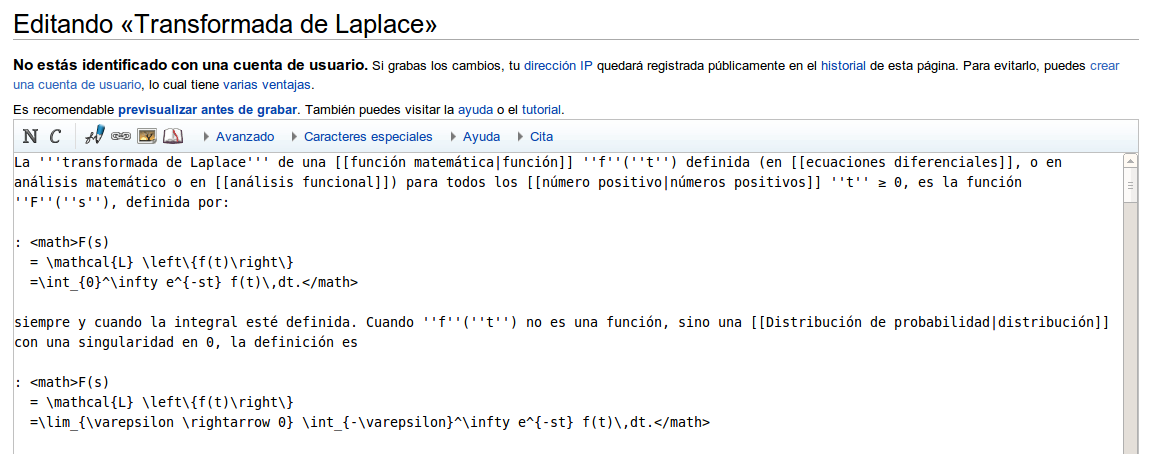
\includegraphics[width=6in]{fig/wiki_markup}
  \caption{Lenguaje Wiki Markup}
  \label{fig:wiki_markup}

\end{figure}


En los últimos años han aparecido en Internet diversos editores WYSIWYG que permiten al usuario modificar de forma inconsciente y en tiempo real el HTML del texto que introducen. Estos editores se sustentan en tecnologías como lenguajes interpretados en el lado del cliente, que ejecutados en un navegador, permiten modificar de forma dinámica el HTML del cuerpo del texto. Si esto es así, ¿por qué se siguen usando lenguajes de etiquetado intermedio?. 

El problema de permitir al usuario introducir directamente código HTML, para ser renderizado posteriormente en la página, presenta un grave riesgo para la seguridad del sistema, es por eso que en un principio se adoptaron lenguajes como BBCode para evitar este tipo de ataques. A este tipo de ataques se les conoce como amenazas XSS, y hacen referencia habitualmente a la inyección de código malicioso en el código de la página.

El trabajo de limpieza del código HTML debe ser exhaustivo, lo que hace de esta una tarea tediosa, por lo que se adoptó el camino fácil del uso de lenguajes intermedios. Es de suma importancia que el análisis del HTML generado en busca de amenazas sea efectivo y se realice de forma correcta, y dada la complejidad de dicha tarea, implementarlo nosotros mismos dentro del marco temporal de este proyecto no es una opción. En lugar de eso existen diversas alternativas en la Web que podemos usar, habiéndonos decantado finalmente por HTMLpurifier~\cite{htmlpurifier}.

El editor resultante es ligero, elegante, fácil de usar y cumple con los requisitos de edición requeridos por la plataforma SWAD. SWADE no busca la potencia de edición de otras alternativas Web como CKEditor~\cite{CKEditor:ckeditor} (al nivel de programas de ofimática como Word), para este tipo de tareas se usarán hojas de estilos CSS. En la figura ~\ref{fig:test1} podemos ver cómo queda el editor integrado en SWAD en la sección mensajes.

\begin{figure}[h!]
  \centering
      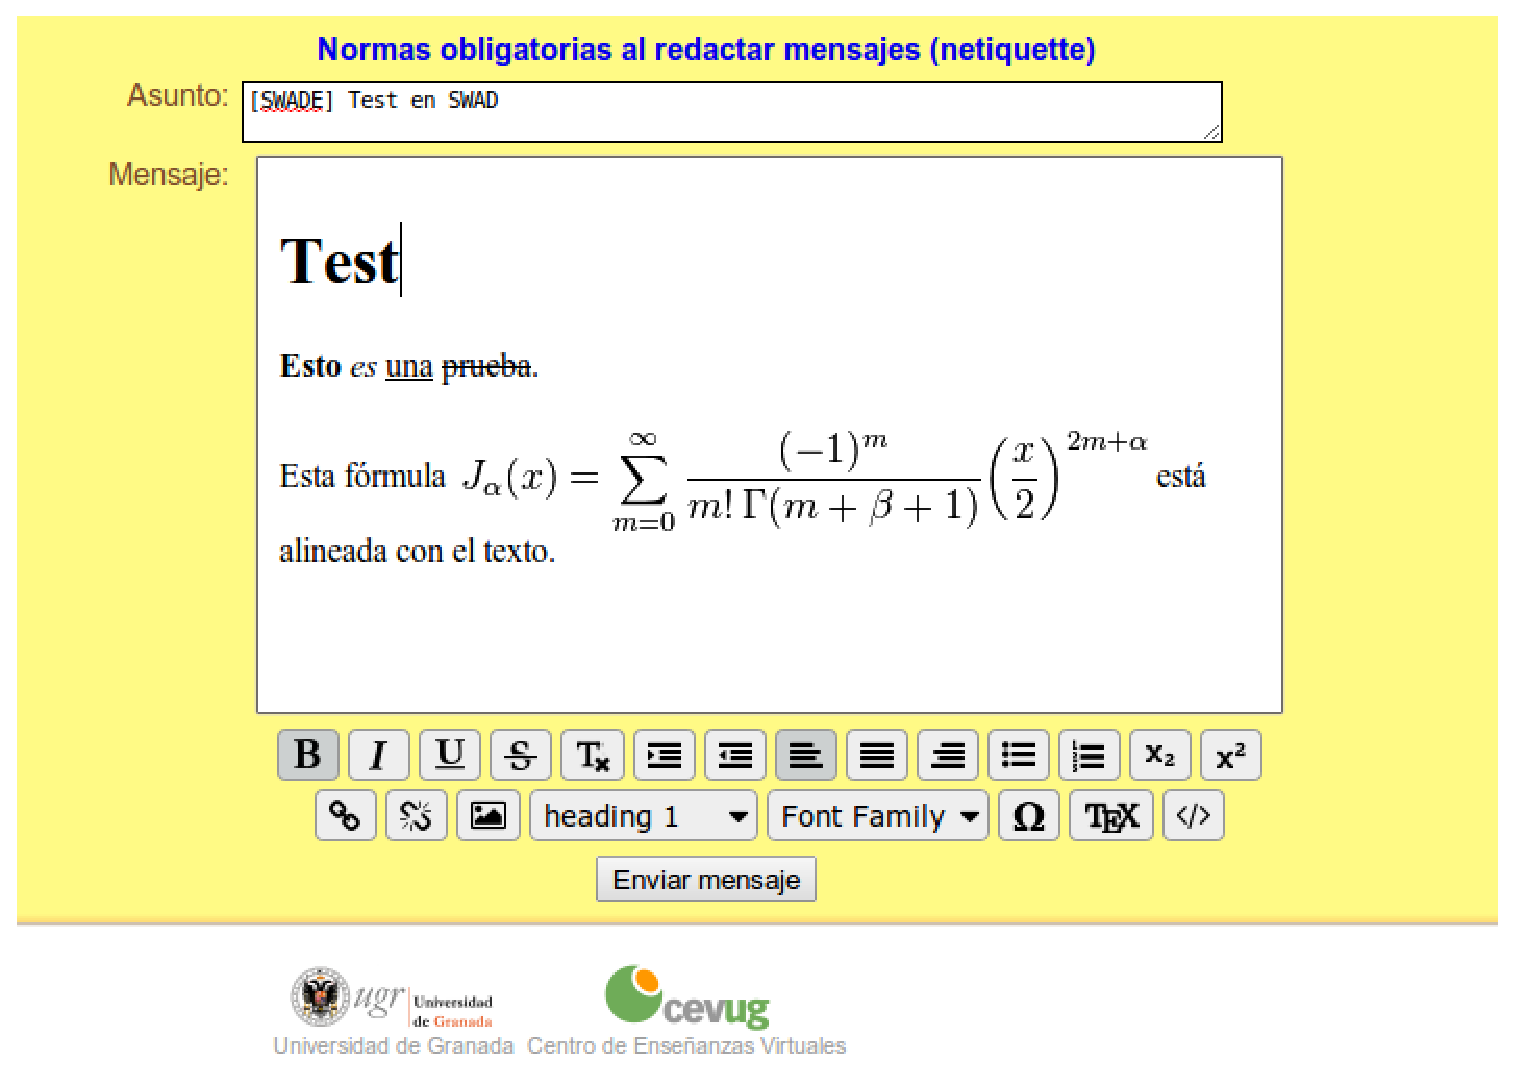
\includegraphics[width=5in]{fig/swade_test1}
  \caption{SWADE en mensajes}
  \label{fig:test1}

\end{figure}


Otra funcionalidad de la que SWAD carece es un editor de fórmulas, de gran importancia cuando se trata de introducir preguntas de tipo test. En este caso nos decantaremos por un editor sencillo basado en LaTeX, que hará indispensable que el usuario tenga unas nociones básicas de dicho lenguaje. En nuestro editor de fórmulas el usuario podrá ver mientras escribe la fórmula que se está formando. Para llevar a cabo esta tarea usamos la herramienta MathJax, que se sustenta en AJAX (Asynchronous Javascript And XML) y hace un renderizado con HTML y CSS de dicha fórmula. Este proceso se realiza en el lado del cliente (navegador web).En la figura ~\ref{fig:test2} podemos ver el editor de fórmulas.


\begin{figure}[h!]
  \centering
      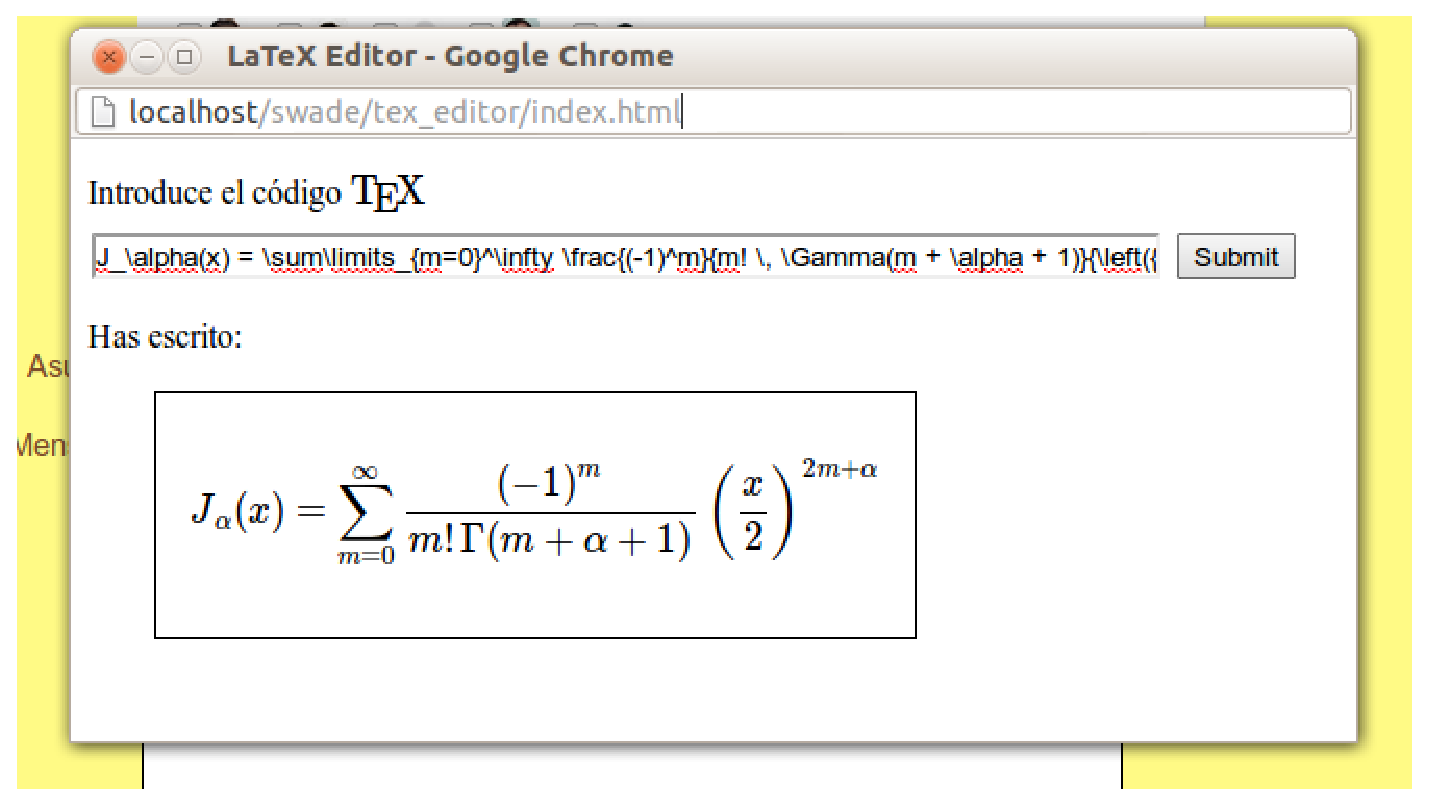
\includegraphics[width=5in]{fig/swade_test2}
  \caption{\rm\TeX\ Editor}
  \label{fig:test2}

\end{figure}

Una vez introducido el código, el usuario confirmará que es la fórmula que quiere enviándose una petición al servidor donde se generará la imagen png correspondiente a la fórmula, usando para esta tarea la herramienta texvc~\cite{texvc}, y devolviéndose finalmente el código HTML necesario para insertar dicha imagen. Esta petición al servidor se realiza de forma asíncrona usando AJAX, de forma que cuando se recibe la respuesta, el editor de fórmulas inserta el código de la imagen en el editor SWADE. 

Se ha tenido en cuenta la posibilidad de edición de una fórmula, por lo que al hacer click en una se nos abrirá el editor de fórmulas permitiéndonos ``editar'' la fórmula. Hay que decir que la imagen no se edita, como era de esperar, sino que se elimina la imagen anterior y se posiciona en su lugar una nueva imagen generada.

 

